\chapter{Исследовательский раздел}
\label{cha:research}

В данном разделе будет проведено функциональное тестирование разработанного программного обеспечения. Также будет проведено измерение каждого из реализованных алгоритмов.

\section{Пример работы}

\section{Технические характеристики}
\begin{itemize}
    \item Процессор: AMD Ryzen 2700 4.00GHz \cite{ryzen}.
    \item Оперативная память: 16GiB.
    \item Операционная система: Linux Kernel 5.14.8 \cite{kernel}.
\end{itemize}

\section{Тестирование}


\section{Время выполнения алгоритмов}

Время выполнения алгоритмов было найдено при помощи библиотеки Google Benchmark [5]. 
Результаты измерения времени (в наносекнудах) были зафиксированы в Таблице \ref{tab:benchmark}.

\begin{table}[ht]
  \caption{Замер времени для строк размером от 1 до 100. }
  \begin{tabular}{|c|c|c|c|c|}
  \hline
  Кол-во элементов & Пузырьком & Пирамидальная  & Поразрядная \\
  \hline
  10  &  $44,383$   &  $128,298$   & $2500,29$            \\
    \hline
  100  & $347,821$   & 568,6785$    & 3163,944         \\
    \hline
  1000  & $13758,153$   & $5469,580$    & 16008,886          \\
    \hline
  10000  & $629640,299$  & $47993,210$   & 140987,35   \\
    \hline
  100000  &  $63081037,797$ & $453011,148$ & 1587590,485\\
   \hline
  \end{tabular}
  \label{tab:benchmark}
\end{table}

\begin{figure}
    \centering
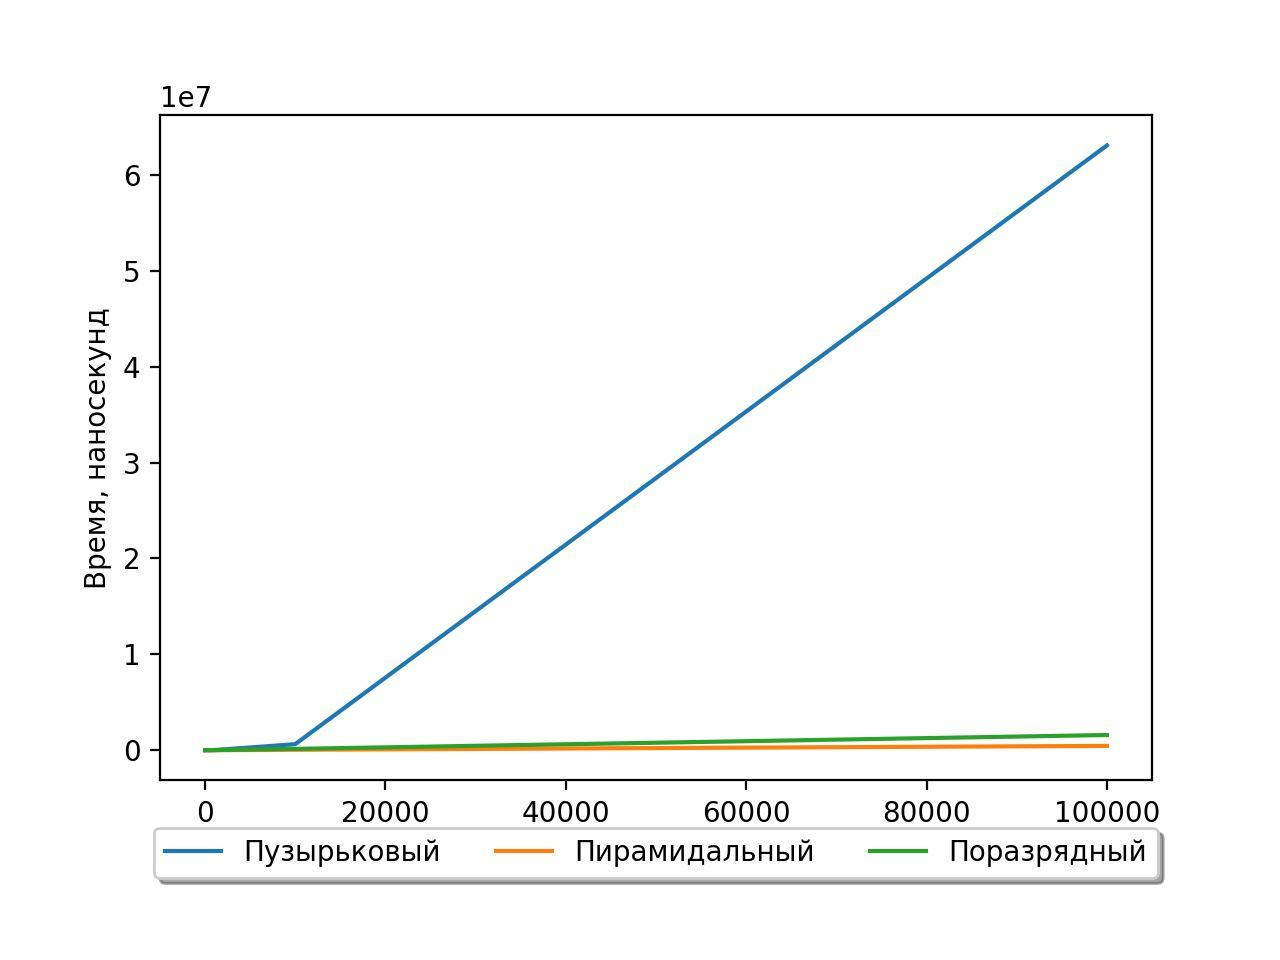
\includegraphics[width=\textwidth]{sem-v-aa-master/lab1/tex/inc/plots/photo_2021-10-31_15-06-34.jpg}

    \caption{Временные характеристики различных реализаций алгоритмов для случайно упорядоченных массивов}
    \label{fig:timestamps}
\end{figure}

\begin{figure}
    \centering
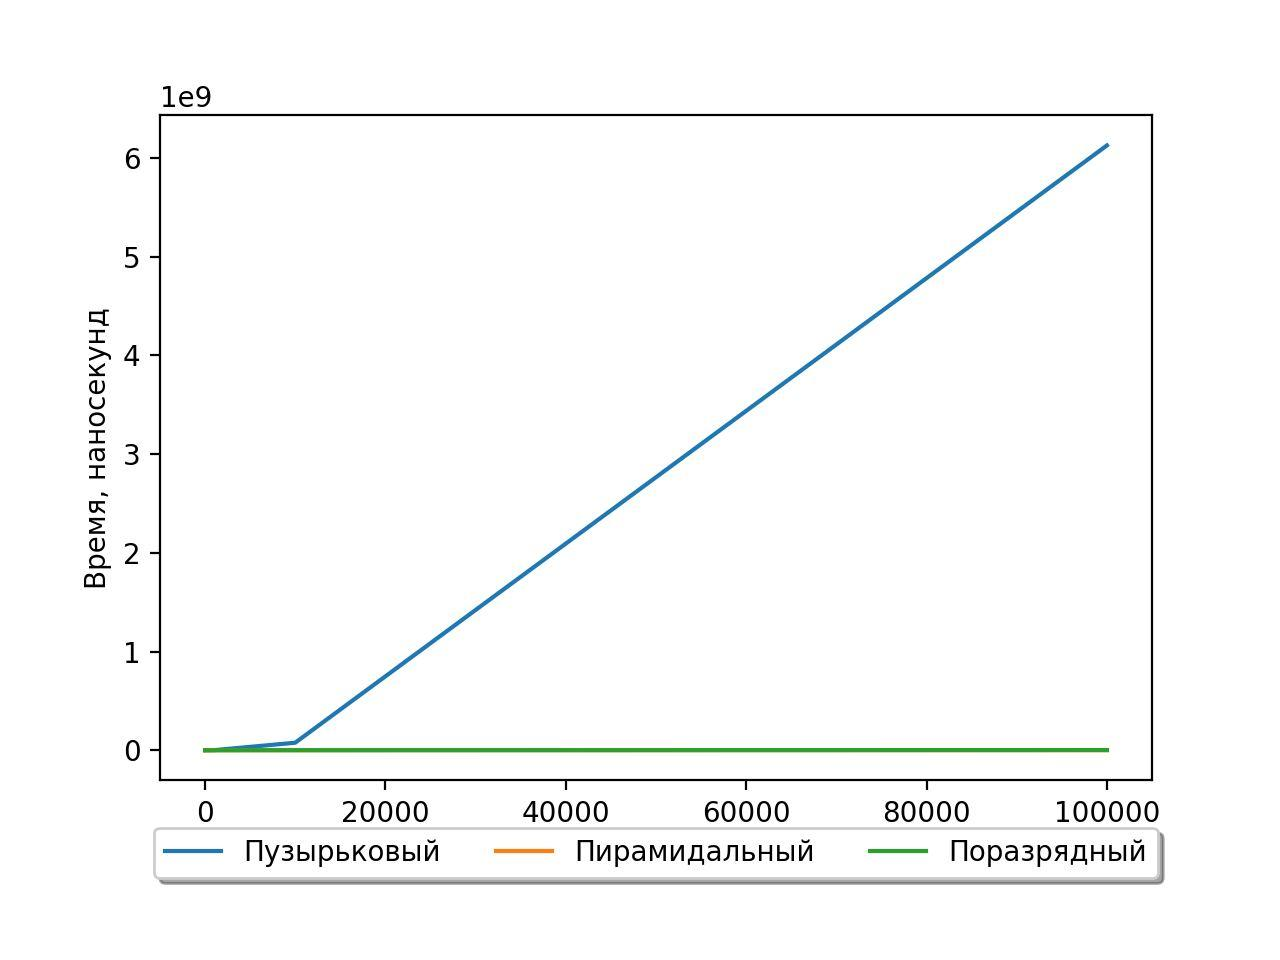
\includegraphics[width=\textwidth]{sem-v-aa-master/lab1/tex/inc/plots/photo_2021-10-31_18-36-28.jpg}

    \caption{Временные характеристики различных реализаций алгоритмов для упорядоченных по убыванию массивов}
    \label{fig:timestamps_descending}
\end{figure}

\begin{figure}
    \centering
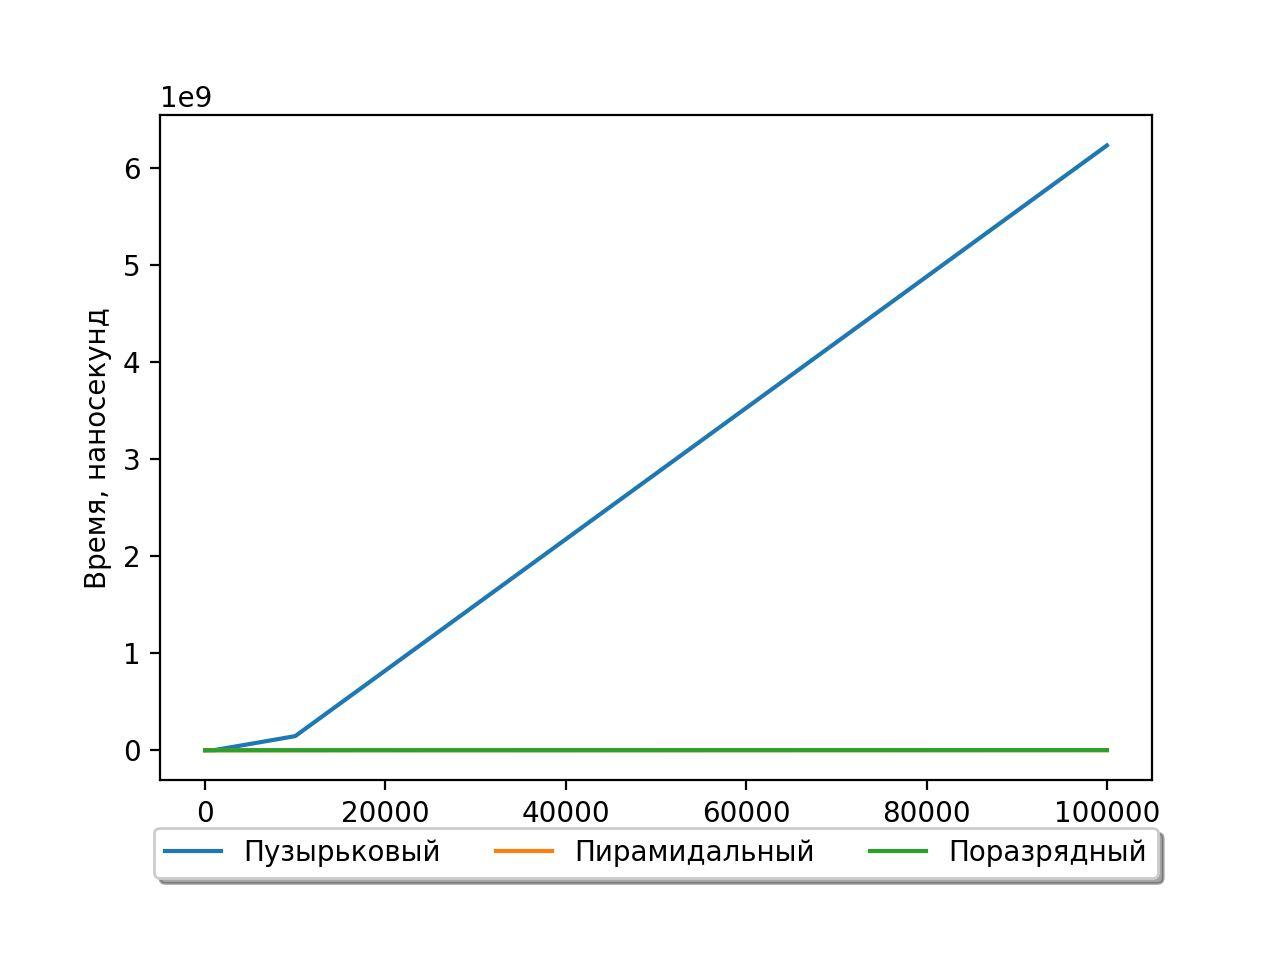
\includegraphics[width=\textwidth]{sem-v-aa-master/lab1/tex/inc/plots/photo_2021-10-31_18-36-32.jpg}

    \caption{Временные характеристики различных реализаций алгоритмов для упорядоченных по возрастанию массивов}
    \label{fig:timestamps_ascending}
\end{figure}

Для рассмотренных значений массива, представленных в таблице \ref{tab:benchmark} в лучшем случае (предупорядоченного по возрастанию массива \ref{fig:timestamps_ascending}) наиболее быстрым на промежутке от 50 до 10000 является пирамидальная сортировка: при размере в массива более 1000 отношение ее к пузырьковой сортировке уже более чем 2.5 раза, а в сравнении с поразрядной сортировкой мы получим преимущество на 3000 наносекунд. Для значений меньших 50 заметное преимущество имеет пузырьковая сортировка. 

В худшем случае (предупорядоченного по убыванию массива \ref{fig:timestamps_descending}) Пузырьковая сортировка на промежутке от 0 до 200 показывает лучший результат. На оставшемся промежутке временная характеристика пузырьковой сортировки значительно уступает пирамидальной и поразрядной сортировке, которые в свою очередь соотносятся друг к другу как $1/2.5 - 1/3$ (в пользу пирамидальной).

В общем случае наиболее эффективной сортировкой на промежутке от 100  до 100000 остается пирамидальная сортировка; в среднем они опрежает поразрядную сортировку в 2-3.5 раза.

\section{Вывод}
В данном разделе были рассмотрены все три сортировки, представленных ранее.

Наиболее времязатратной сортировкой оказалась пузырьковая, что и было теоретически доказано в конструкторском разделе. Самой эффективной оказалась пирамидальная сортировка, опередившая две остальные на рассмотренном интервале размеров массива, лишь уступая пузырьковой на интервале от 0 до 100.
%%% Local Variables:
%%% mode: latex
%%% TeX-master: "rpz"
%%% End:
